\documentclass[a4paper, 12pt]{report}

\usepackage[utf8]{inputenc}
\usepackage[french]{babel}
%\usepackage[english]{babel}
\usepackage[T1]{fontenc}
% \usepackage[latin1]{inputenc}

\usepackage[top=3cm, bottom=3cm, left=2.3cm,right=2cm]{geometry}
\usepackage{graphicx}
\usepackage{color}
\usepackage{titlepic}
\usepackage{hyperref}
\usepackage{url}
\usepackage[table]{xcolor}
\definecolor{light-gray}{gray}{0.50}
\definecolor{very-light-gray}{gray}{0.9}

\usepackage{listings}
\lstset{language=python, 
  basicstyle=\scriptsize, 
  numbers=left,
  numberstyle=\tiny\color{light-gray},  % the style that is used for the line-numbers
  numbersep=5pt,                  % how far the line-numbers are from the code
  backgroundcolor=\color{white},      % choose the background color. You must add \usepackage{color}
  showspaces=false,               % show spaces adding particular underscores
  showstringspaces=false,         % underline spaces within strings
  showtabs=false,                 % show tabs within strings adding particular underscores
  frame=single,                   % adds a frame around the code
  %rulecolor=\color{black},        % if not set, the frame-color may be changed on line-breaks within not-black text (e.g. commens (green here))
  tabsize=4,                      % sets default tabsize to 2 spaces
  captionpos=b,                   % sets the caption-position to bottom
  breaklines=true,                % sets automatic line breaking
  breakatwhitespace=false,        % sets if automatic breaks should only happen at whitespace
  title=\lstname,                   % show the filename of files included with \lstinputlisting;
                                  % also try caption instead of title
  %keywordstyle=\color{blue},          % keyword style
  commentstyle=\color{light-gray},       % comment style
  %stringstyle=\color{yellow}         % string literal style
}

%en-tete de page
\usepackage{fancyhdr}
\lhead{MLBD}
\chead{Casas \& Cogno}
\rhead{\today}
\pagestyle{fancy}

%\renewcommand{\thesection}{\arabic{section}} % pour numerotation des sections

\titlepic{
\includegraphics[width=0.5\textwidth]{img/mse_logo.jpg}}
\title{\huge{HES-SO Master} \\ \Huge{\textbf{\textsc{MLBD}}} \\
\LARGE{Machine Learning on Big Data} \\
\vspace{2cm} \huge{\textbf{Projet}} \\ 
\huge{Catégorisation de films}}
\author{\\ \\ Simone \textsc{Cogno} \& Jacky \textsc{Casas} \\
\\ \\
Professeurs : Carlos \textsc{Pena} \& Andres \textsc{Perez-Uribe} \\
Assistant : Julien \textsc{Rebetez}}
\date{\today}


\begin{document}
\maketitle % page de garde
\newpage
\tableofcontents
%\newpage

\chapter{Introduction}

\section{Contexte}

Ce projet s'insère dans le cadre du cours ``Machine Learning on Big Data'' (ou MLBD) du Master HES-SO. Durant ce cours, plusieurs techniques de machine learning ont été enseignées dans le but de donner une idées de ce qui se fait dans l'industrie dans ce domaine. \\

Le ``machine learning'' ou ``apprentissage automatique'', un des champs d'étude de l'intelligence artificielle, est la discipline scientifique concernée par le développement, l'analyse et l'implémentation de méthodes automatisables qui permettent à une machine (au sens large) d'évoluer grâce à un processus d'apprentissage, et ainsi de remplir des tâches qu'il est difficile ou impossible de remplir par des moyens algorithmiques plus classiques.\footnote{\url{http://fr.wikipedia.org/wiki/Apprentissage\_automatique}} \\


Le but de ce projet est de classifier des films grâce à leur synopsis. Pour ce faire, nous utiliserons la technique dite des cartes auto organistarices. En anglais, cette technique est connue sous le nom de self organizing maps (SOM).\footnote{\url{http://fr.wikipedia.org/wiki/Carte\_auto\_adaptative}} On la connaît aussi sous le nom de cartes de Kohonen. Il s'agit de méthodes d'apprentissage non-supervisées\footnote{\url{http://fr.wikipedia.org/wiki/Apprentissage\_non\_supervis\%C3\%A9}} basées sur des réseaux de neurones artificiels. Un apprentissage non-supervisé signifie qu'une quantité de données est fournie au système et en sortie nous obtenons un modèle qui groupe les différentes données selon leurs affinités ou leur ressemblances. Cette méthode est utilisée notamment pour faire de la classification, ce qui est exactement notre but ici.

\newpage
\section{Le projet}

A partir d'une liste de films, nous allons donc chercher sur internet des résumés (ou synopsis) de différents films. Nous allons traiter ces synopsis pour en extraire différentes informations comme les mots présents et leurs occurrences. Grâce à ces informations, nous pourrons contruire une matrice qu'on donnera à notre réseau de neurone pour qu'il nous confectionne une carte auto-organisée qui classifie les différents films.\\

Le but ici est de voir si les classifications que nous créerons sont cohérentes avec les catégories et genres indiqués par les sites comme IMDb. Au fur et à mesure du projet, nous améliorerons les techniques pour avoir des résultats de plus en plus cohérents et pour finir nous donnerons des pistes d'améliorations futures.


\chapter{Démarche}
%---------------------------------------------------------------------------------------------------------------
\section{Liste des films}

Tout d'abord, nous avons trouvé une liste de films qui provient du site \url{IMDb.com}. Elle contient des informations sur 3393 films connus. Cela nous permet d'avoir une liste fixe et de ne pas avoir besoin d'aller les chercher à chaque fois sur internet. Nous avons donc stocké ce fichier que nous utiliserons par la suite. Ce fichier est formaté de la manière suivante : une ligne correspond à un film, chaque ligne contient 5 informations sur le film : \\

\begin{itemize}
 \item Le titre du film
 \item L'année de sortie du film
 \item La note qu'à le film sur IMDb
 \item Le nombre de vote qu'à reçu le film sur IMDb
 \item Le genre (plusieurs genres séparés par des virgules)
\end{itemize}

\vspace{0.4cm}
Chacune des ces cinq informations est séparée par deux espaces. Voici un aperçu de cette structure de fichier : \\

\begin{lstlisting}[language=bash]
  The Pianist  2002  8.5  151864  Biography,Drama,War
  The Godfather  1972  9.2  450433  Crime,Drama,Thriller
  Casper  1995  5.7  28316  Comedy,Family,Fantasy
  Hostel  2005  5.7  69499  Mystery,Thriller
  Juno  2007  7.8  163142  Comedy,Drama,Romance
\end{lstlisting}

Cette structure nous permet donc d'extraire facilement les informations voulues avec la fonction Python suivante : \\

\begin{lstlisting}[language=python]
  def extractMovieList(fname):

      with open(fname) as f:
          content = f.readlines()
    
      title = []
      year = []
      grade = []
      votes = []
      genre = []

      for line in content:
          infos = line.split('  ')
          title.append(infos[0].replace('"',''))
          year.append(infos[1])
          grade.append(infos[2])
          votes.append(infos[3])
          genre.append(infos[4])

      return [title, year, grade, genre]
\end{lstlisting}

%---------------------------------------------------------------------------------------------------------------
\section{Recherche d'information sur un film}

Les données disponibles dans le fichier \texttt{movielist.txt} ne nous permetteront pas de classifier les films. C'est juste une liste qui nous permet d'avoir une quantité de titre de films ainsi que les genres de chaque film. Nous voulons alors rechercher les descriptifs de chaque film. Pour cela, nous utilisons une API\footnote{\url{http://fr.wikipedia.org/wiki/Interface\_de\_programmation}} d'IMDb qui est documentée à l'adresse \url{http://omdbapi.com}. Cette API nous permet de chercher des informations sur un film soit en donnant le titre, soit en donnant l'identitiant IMDb du film (ce que nous n'avons pas). 

Nous allons alors prendre la liste de films et faire une requête sur cette API pour chaque titre de film que nous avons. De temps en temps, aucun résultat ne sort, nous passons simplement au suivant. Nous enregistrons alors tous les résultats dans un fichier sous format JSON.\footnote{\url{http://fr.wikipedia.org/wiki/JavaScript\_Object\_Notation}} \\

\begin{lstlisting}[language=python]
  def getMovieDescriptions(movieTitles, fname):

      movieInfos = []
      base_url = "http://www.omdbapi.com/?plot=full&r=json&t="
    
      for title in movieTitles:
          print 'fetching ' + title
          url = base_url + title
          r = requests.get(url)
          movieInfos.append(r.json())

      with open(fname, 'wb') as outfile:
          json.dump(movieInfos, outfile)
\end{lstlisting}

Pour chaque film, nous recevons différentes informations, dont un lien vers une image, le titre, la durée du film, l'année, les acteurs, le pays, la langue, l'identifiant IMDb, un descriptif, etc. Ce qui nous intéresse à première vue est le descriptif. Seulement après avoir analysé ces descriptifs, nous remarquons qu'ils sont souvent courts, ils comportent pour la plupart moins de cinquante mots. Cela est beaucoup trop peu pour pouvoir trouver des ressemblances entres les films et les classifier. 

Nous avons alors eu l'idée d'utiliser l'identifiant IMDb de chaque films pour aller chercher plus d'informations sur les films. Après quelques recherches, nous trouvons qu'il y a une page spécifique pour chaque film sur le site IMDb où se trouve un résumé plus détaillé du film. L'adresse est formée de la façon suivante : \textit{'http://www.imdb.com/title/[imdbId]/synopsis'}. Il nous reste donc à remplacer l'identifiant que l'on veut dans cette URL et nous arrivons sur un beau descriptif, qu'il faut tout de même extraire de la page web (parser du HTML est toujours une partie de plaisir, quoique).

Un script Python va nous permettre d'aller chercher le descriptif de chaque film et de l'enregistrer cette fois dans un fichier séparé pour chaque film. Voici ce script : \\

\lstinputlisting[language=Python]{code/fetchSynopsis.py}

Tous les films n'avaient pas leur page de descriptif correspondante. Sur les 3393 films initiaux, seuls 2396 ont pu être extrait et enregistré. C'est tout de même assez pour faire nos tests. Nous continuons donc avec cela.

%---------------------------------------------------------------------------------------------------------------
\section{Création du dataset}

Nous avons maintenant tout en main, et en local, pour pouvoir générer les structures de données spécifiques. Nous avons besoin de trois structures différentes :

\begin{itemize}
 \item un vecteur contenant la liste des films
 \item un vecteur contenant la liste de tous les mots qui apparaissent dans les textes de description 
 \item une matrix contenant le nombre d'occurrence de chaque mot pour chaque film. Chaque ligne correspond à un film et chaque colonne à un mot.
\end{itemize}

\vspace{0.4cm}
%\lstinputlisting[language=Python]{code/formatData.py}
Voici comment la liste des titres de film est générée : \\

\begin{lstlisting}[language=python]
  def formatTitle(data):
      print 'Generating title list...'
      titles = []
      i = 0;
      for movie in data:
          fname = 'data2/synopsis/' + movie['imdbID'] + '.txt'
          # if synopsis file exists
          if os.path.isfile(fname):
              titles.append(movie['Title'])
              i = i + 1
      print 'There is ' + str(i) + ' movies.'
      return titles
\end{lstlisting}

Il a fallu ensuite générer la liste de tous les mots qui apparaissent dans les descriptifs de chaque film. Là il fallait faire plusieurs traitement pour enlever la ponctuation et surtout enlever les \textit{``stop words''} (ou \textit{``mots vides''} en français) qui sont les mots qui n'ont pas vraiment de valeur comme les déterminants, les pronoms. Ces mots apparaissent avec une fréquence contante dans les différents textes et n'ont donc pas de valeur dans la distinction entre les textes. Pour ce faire, nous avons utilisé la librairie python \texttt{nltk}. Nous avons ensuite fait une liste des mots uniques restants. Voici le code correspondant : \\

\begin{lstlisting}[language=python]
  def formatWords(data):
      print 'Generating word list...'
      words = []
      for movie in data:
          fname = 'data2/synopsis/' + movie['imdbID'] + '.txt'
          # if synopsis file exists
          if os.path.isfile(fname):
              synopsis = ''
              with open(fname, 'r') as thefile:
                  synopsis = thefile.read().replace('\n', '')

              synopsis = synopsis.lower()
              # clean words
              word_list = re.findall(r'\w+', synopsis, flags = re.UNICODE | re.LOCALE) 
              # remove the stopwords
              word_list = filter(lambda x: x not in stopwords.words('english'), word_list)
              for word in word_list:
                  #word = clean(word)
                  if word not in words:
                      words.append(word)
      print 'There is ', len(words), ' words in the list.'
      return words
\end{lstlisting}

La partie la plus difficile est de générer la matrice indiquant combien de fois chaque mot apparaît dans chaque texte. Il a fallu optimiser le maximum ce traitement car il prend énormément de temps à l'exécution. Et voici donc comment la matrice est générée : \\

\begin{lstlisting}[language=python]
  def generateMatrix(data, words):
      print 'Generating matrix...'
      matrix = []
      i = 0
    
      for movie in data:
          i = i + 1
          fname = 'data2/synopsis/' + movie['imdbID'] + '.txt'
          # if synopsis file exists
          if os.path.isfile(fname):
              print 'movie ' + str(i) + ' on ' + str(len(data))
              line = []
              synopsis = ''
              with open(fname, 'r') as thefile:
                  synopsis = thefile.read().replace('\n', '')

              synopsis = synopsis.lower()
              word_list = re.findall(r'\w+', synopsis, flags = re.UNICODE | re.LOCALE) 
              word_list = filter(lambda x: x not in stopwords.words('english'), word_list)
              for word in words:
                  count = 0

                  for w in word_list:
                      if w == word:
                          count = count + 1
                  line.append(count)

              matrix.append(line)
          else :
              print 'movie ' + str(i) + ' has no synopsis'
      print 'Done.'
      return matrix
\end{lstlisting}

Avec ces trois matrices, nous pouvons directement faire marcher les Self-Organizing Maps, mais après plusieurs essais, nous nous sommes rendu compte que les résultats n'étaient pas très parlant.

%---------------------------------------------------------------------------------------------------------------
\section{Optimisations}

Une première amélioration a été de supprimer les mots qui n'apparaissent que dans un seul film. En effet, ces mots n'ont pas de valeur (au même titre que les stopwords) car ils ne permettent pas de faire des corrélations entre différents films. Nous avons donc fait un premier traitement qui supprime ces mots. Il a donc fallu supprimer ces mots de la liste des mots, mais étalement supprimer toutes les colonnes de la matrice correspondantes à ces mots. Grâce à la librairie \texttt{Numpy}, ce traitement est assez peu gourmand en nombre de lignes de code. Nous utilisons un masque pour filtrer les résultats. \\

\begin{lstlisting}[language=python]
  def removeLonelyWords(words, matrix):

      word_counts = matrix.sum(axis=0)
      word_mask = word_counts > 1

      # convert words to numpy array
      words = np.array(words)

      matrix = matrix[:,word_mask]
      words = words[word_mask]

      return words.tolist(), matrix
\end{lstlisting}

Les résultats générés avec ces matrices n'était toujours pas suffisant pour classifier de manière optimale les films. Nous avons alors appliqué l'algorithme TF-IDF\footnote{\url{http://fr.wikipedia.org/wiki/TF-IDF}} (\textit{Term Frequency-Inverse Document Frequency}) à la matrice. Cet algorithme permet d'évaluer l'importance d'un mot contenu dans un texte, relativement à une série de textes. Voici les formules correspondantes :

\[idf_i = log\frac{N}{t_j : w_i \in t_j}\]
\[tfidf_{ij} = tf_{ij} \cdot idf_i\]

Le terme $tf_{ij}$ est la matrice avec la fréquence de mots dans chaque texte que nous avons déjà générée. $N$ est le nombre total de textes. $t_j$ est le nombre de textes où le mot $w_i$ apparaît. $tfidf_{ij}$ est la matrice finale, obtenue avec l'algorithme TF-IDF. Nous allons utiliser cette matrice en remplacement de la précédente pour générer la carte de Kohonen. Voici le code qui permet cette optimisation : \\

\begin{lstlisting}[language=python] 
 def applyTFIDF(matrix):

      tf = matrix
      N = matrix.shape[0]
      matrix_mask = matrix > 0
      nf = matrix_mask.sum(axis=0)
      idf = np.log10(nf*(1.0/N))
      tfidf = tf * idf

      return tfidf
\end{lstlisting}

Lors de la sauvegarde du fichier contenant les deux vecteurs et la matrice, nous passons d'un fichier de 287.7Mo à un fichier de 581.7Mo. Il y a au total 39404 mots différents pour 2396 films. Cela est dû au fait que les valeurs de la matrice sont des nombres à virgules à la place de simples entiers.

%---------------------------------------------------------------------------------------------------------------
\section{Matrice de distances}

\label{matrice-distance}
Pour avoir une notion de distance entre les documents nous avons créé une matrice des distances. Pour faire cela, on a utilisé la librairie "hcluster" \footnote{Hcluster, \url{https://code.google.com/p/scipy-cluster/}} qui prend en entrée une matrice de vecteurs des documents et elle permet de définir une métrique de distance : dans notre cas on a utilisé la fonction "cosine".

Le code pour la génération de la matrice de distance est le suivant : \\

\begin{lstlisting}[language=python]
  titles, words, matrix = extractArrays(infos)
  distanceMatrix = pairwise_distances(matrix, metric='cosine')
\end{lstlisting}


%---------------------------------------------------------------------------------------------------------------
\section{Liste des films similaires}

Pour voir si la matrice des vecteurs des documents décrit bien les documents nous avons implémenté une fonction qui, avec un film en paramètre, retourne les N films las plus similaires à celui-ci.

La fonction prend en paramètre l'id du film initial, le nombre des films similaires à afficher, la matrice de distance décrite dans la section \ref{matrice-distance} ainsi que le vecteur des titres des films.

Le code de cette fonction est le suivant : \\

\begin{lstlisting}[language=python]
  def printClosest(idxFilm, numclosest, distanceMatrix, titles):
    print titles[idxFilm]+":"
    cloasest= heapq.nsmallest(numclosest,range(len(distanceMatrix[idxFilm])),distanceMatrix[idxFilm].take)
    for idx, val in enumerate(cloasest):
        print  "\t"+str(idx)+" "+titles[val]
\end{lstlisting}


%---------------------------------------------------------------------------------------------------------------
\section{Clustering hiérarchique}

Une fois avoir évalué quelques films avec la liste des films similaires on a voulu vérifier mieux cela en faisan un clastering hiérarchique en vérifiant que les filmes regroupé dans un clastering sont une catégorie similaire.

Pour faire cela, on utilise la libraire "hcluster" pour effectuer le clustering hiérarchique en se basant sur la matrice de distances.

Le clustering hiérarchique sera visualisé dans un dendrogram représentant les regroupements des films. \\

\begin{lstlisting}[language=python]
  Z=linkage(distanceMatrix,method='average')#,method='centroid')
  print Z.shape
  image=dendrogram(Z,labels=titlesCat, distance_sort='descendent',
         leaf_font_size=2, orientation='left', show_contracted=False)
  pylab.savefig("images/clustering100_tf_idf.png",dpi=300,bbox_inches='tight')	 	  
\end{lstlisting}

Pour nous aider à la visualisation du graphique on a utilisé une fonction utilitaire pour visionner les films les plus similaires que sont regroupé par l'algorithme de clustering.

Pour faire cela on a fait la fonction suivante : \\

\begin{lstlisting}[language=python]
  print "first closest cluster"
  for idx in range(10):
      lenTitle=len(titles)
      if (int(Z[idx,0])<lenTitle) & (int(Z[idx,1])<lenTitle):
          print "itr "+str(idx)+":\n"+titlesCat[int(Z[idx,0])]+" "+titlesCat[int(Z[idx,1])]
\end{lstlisting}

La variable Z a été calculée par la fonction de la libraire "hcluter" et on peut voir, à chaque itération, quel film a été mis ensemble avec quelle outre.	


%---------------------------------------------------------------------------------------------------------------
\section{Map de Kohonen}

Une fois avoir vu les résultats depuis le clustering hiérarchique on peut analyser la matrice initiale avec un algorithme un peu plus avancé et qui donne des résultats plus visuels.

On a utilisé l'algorithme de Khonen qui prend en entrée notre matrice des vecteurs des documents et produise en sortie une map en couleur avec la position de chaque filme par rapport a les autres. Les couleurs de la map représente la distance entre chaque film. 

Pour faire cela, on a utilisé la base du code fait dans le TP 
4 \footnote{TP Kohonen, HES-SO, \url{http://193.134.218.37/labs/lab4/lab4_assignment.html}}. Dans celui-là  on a modifié la métrique de mesure de la distance et la construction de la matrice initiale : \\

\begin{lstlisting}[language=python]
  # define cosine metric for configure distance metrix on kohonen
  def cosine_metric(x, y):
      # Returns the cosine distance between x and y.
      nx = np.sqrt(np.sum(x * x, axis=-1))
      ny = np.sqrt(np.sum(y * y, axis=-1))
      # the cosine metric returns 1 when the args are equal, 0 when they are
      # orthogonal, and -1 when they are opposite. we want the opposite effect,
      # and we want to make sure the results are always nonnegative.
      return 1 - np.sum(x * y, axis=-1) / nx / ny

  params = kohonen.Parameters(dimension=len(words), shape=(side,side*2), metric=cosine_metric)
  kmap = kohonen.Map(params)
\end{lstlisting}




%---------------------------------------------------------------------------------------------------------------
% Code integration example
%\begin{lstlisting}[language=bash]
%  sudo apt-get update
%  sudo apt-get install drupal7
%\end{lstlisting}

% Image integration example
%\begin{figure}[h]
%  \centering
%    \includegraphics[width=1\linewidth]{img/drupalFirstPage.png}
%  \caption{Page d'accueil du site créé avec Drupal sur une instance EC2}
%  \label{drupalfirstpage}
%\end{figure}

% Image side-by-side
%\begin{figure}[h!]
%    \centering
%    \begin{tabular}{cccc}
%      \includegraphics[width=.14\linewidth]{randomTree_n5.png} &
%      \includegraphics[width=.22\linewidth]{randomTree_n10.png} &
%      \includegraphics[width=.22\linewidth]{randomTree_n15.png} \\
%      (a) & (b) & (c)\\
%    \end{tabular}
%    \caption{Arbres aléatoires où (a) n=5 (b) n=10 (c) n=15
%    \label{randomTrees}}
%\end{figure}
\chapter{Résultats obtenu}
%---------------------------------------------------------------------------------------------------------------
\section{Liste films similaire}

Les résultats de la liste des film similaire à "Witness for the Prosecution" sont les suivantes :

\begin{lstlisting}[language=python]
  Witness for the Prosecution:Crime,Drama,Mystery,Thriller :

  0 Witness for the Prosecution:Crime,Drama,Mystery,Thriller

  1 A Few Good Men:Crime,Drama,Mystery,Thriller

  2 Touch of Evil:Crime,Film-Noir,Thriller

  3 Chaplin:Biography,Drama

  4 Breaking the Waves:Drama,Romance

  5 Before the Devil Knows Youre Dead:Crime,Drama,Thriller

  6 Mercury Rising:Action,Crime,Drama,Thriller

  7 The Graduate:Comedy,Drama,Romance

  8 Scary Movie:Comedy

  9 Femme Fatale:Crime,Thriller
\end{lstlisting}

On peut voir que la catégorie du film sélectionné est "Crime,Drama,Mystery,Thriller" et on voit que le film détecté comme similaire ont des catégories en commun. On peut en déduire que l'algorithme semble reconnaitre assai bien les films similaires.

%---------------------------------------------------------------------------------------------------------------
\newpage
\section{Clustering hiérarchique}

	Les résultats du clustering hiérarchique sont montrés dans l'image ci-dessous :
	\begin{figure}[h]
	  \centering
	    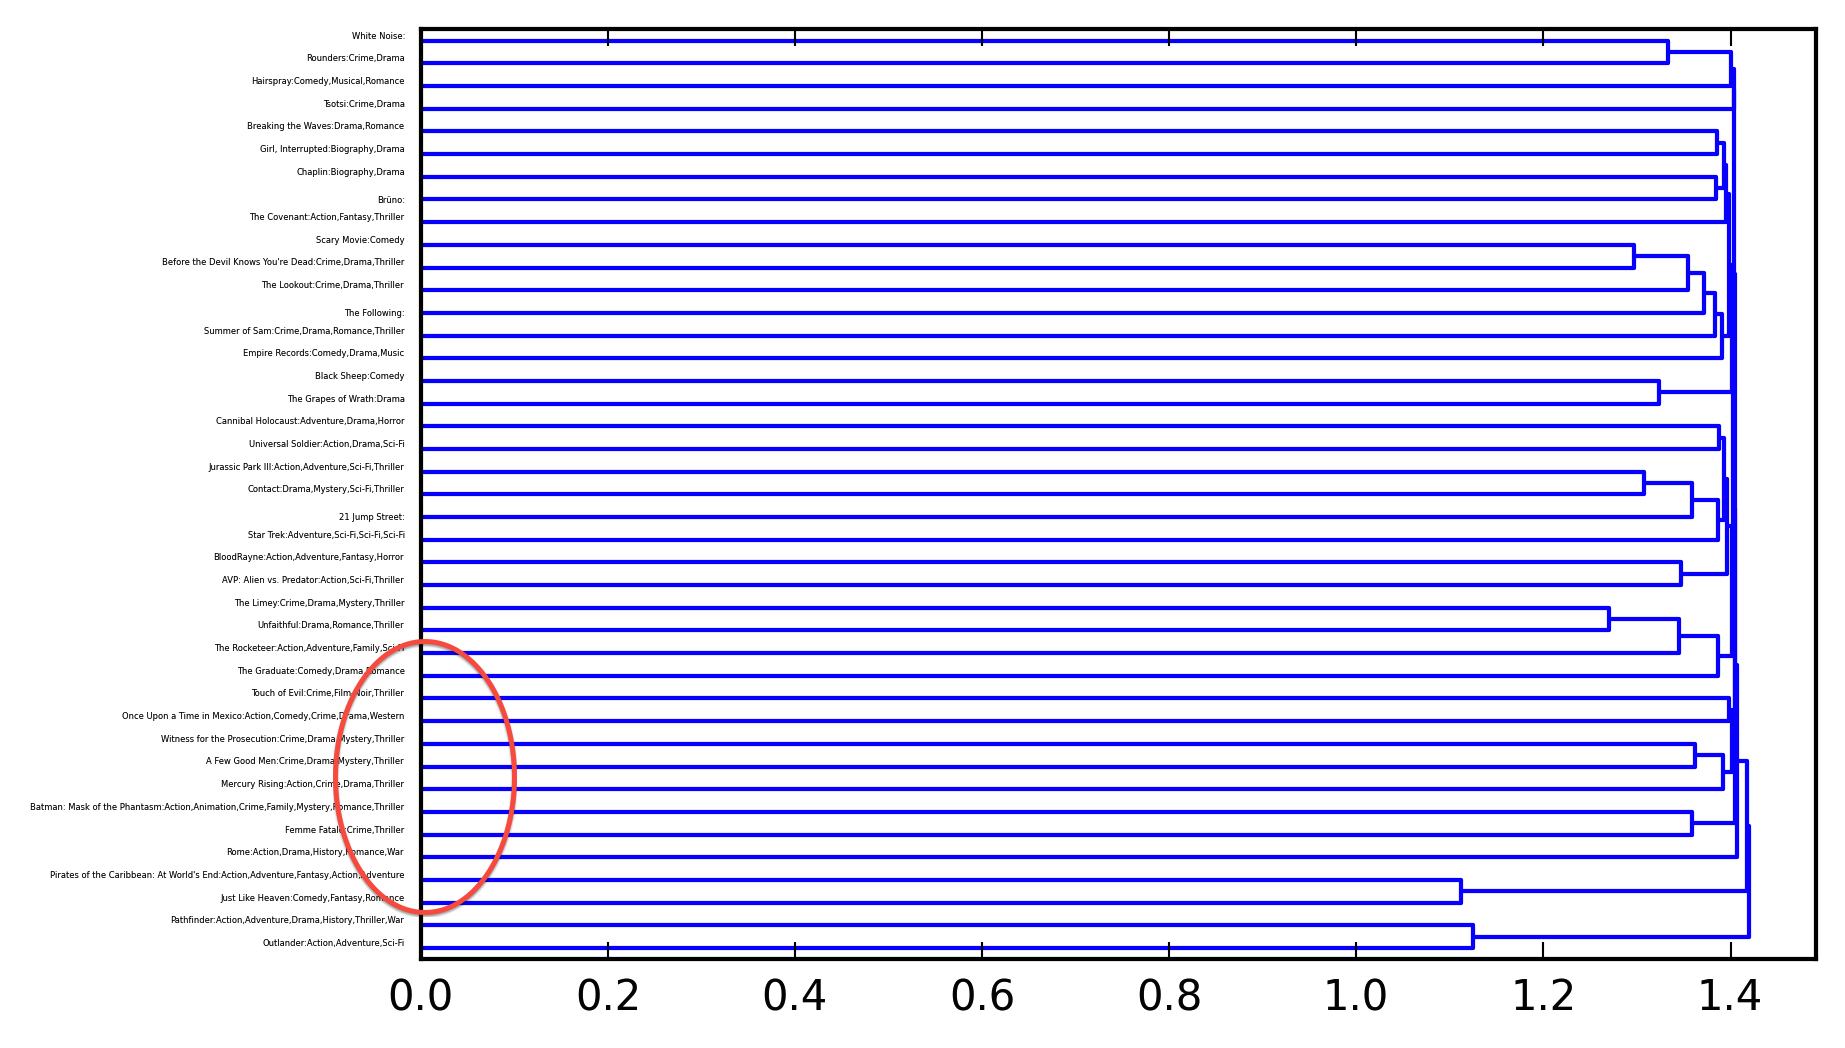
\includegraphics[width=0.6\linewidth]{img/clustering50_tf_idf.png}
	  \caption{Dendogram du clustering hiérarchique}
	  \label{hierarchical}
	\end{figure}
	
	En faisan un zoom sur limage (figure \ref{zoom}) on peut voire quel film a été groupé et on peut voire sa catégorie. Dans l'image ci-dessous on peut voir comme le film de la même catégorie ont été groupé ensemble.
		\begin{figure}[h]
		  \centering
		    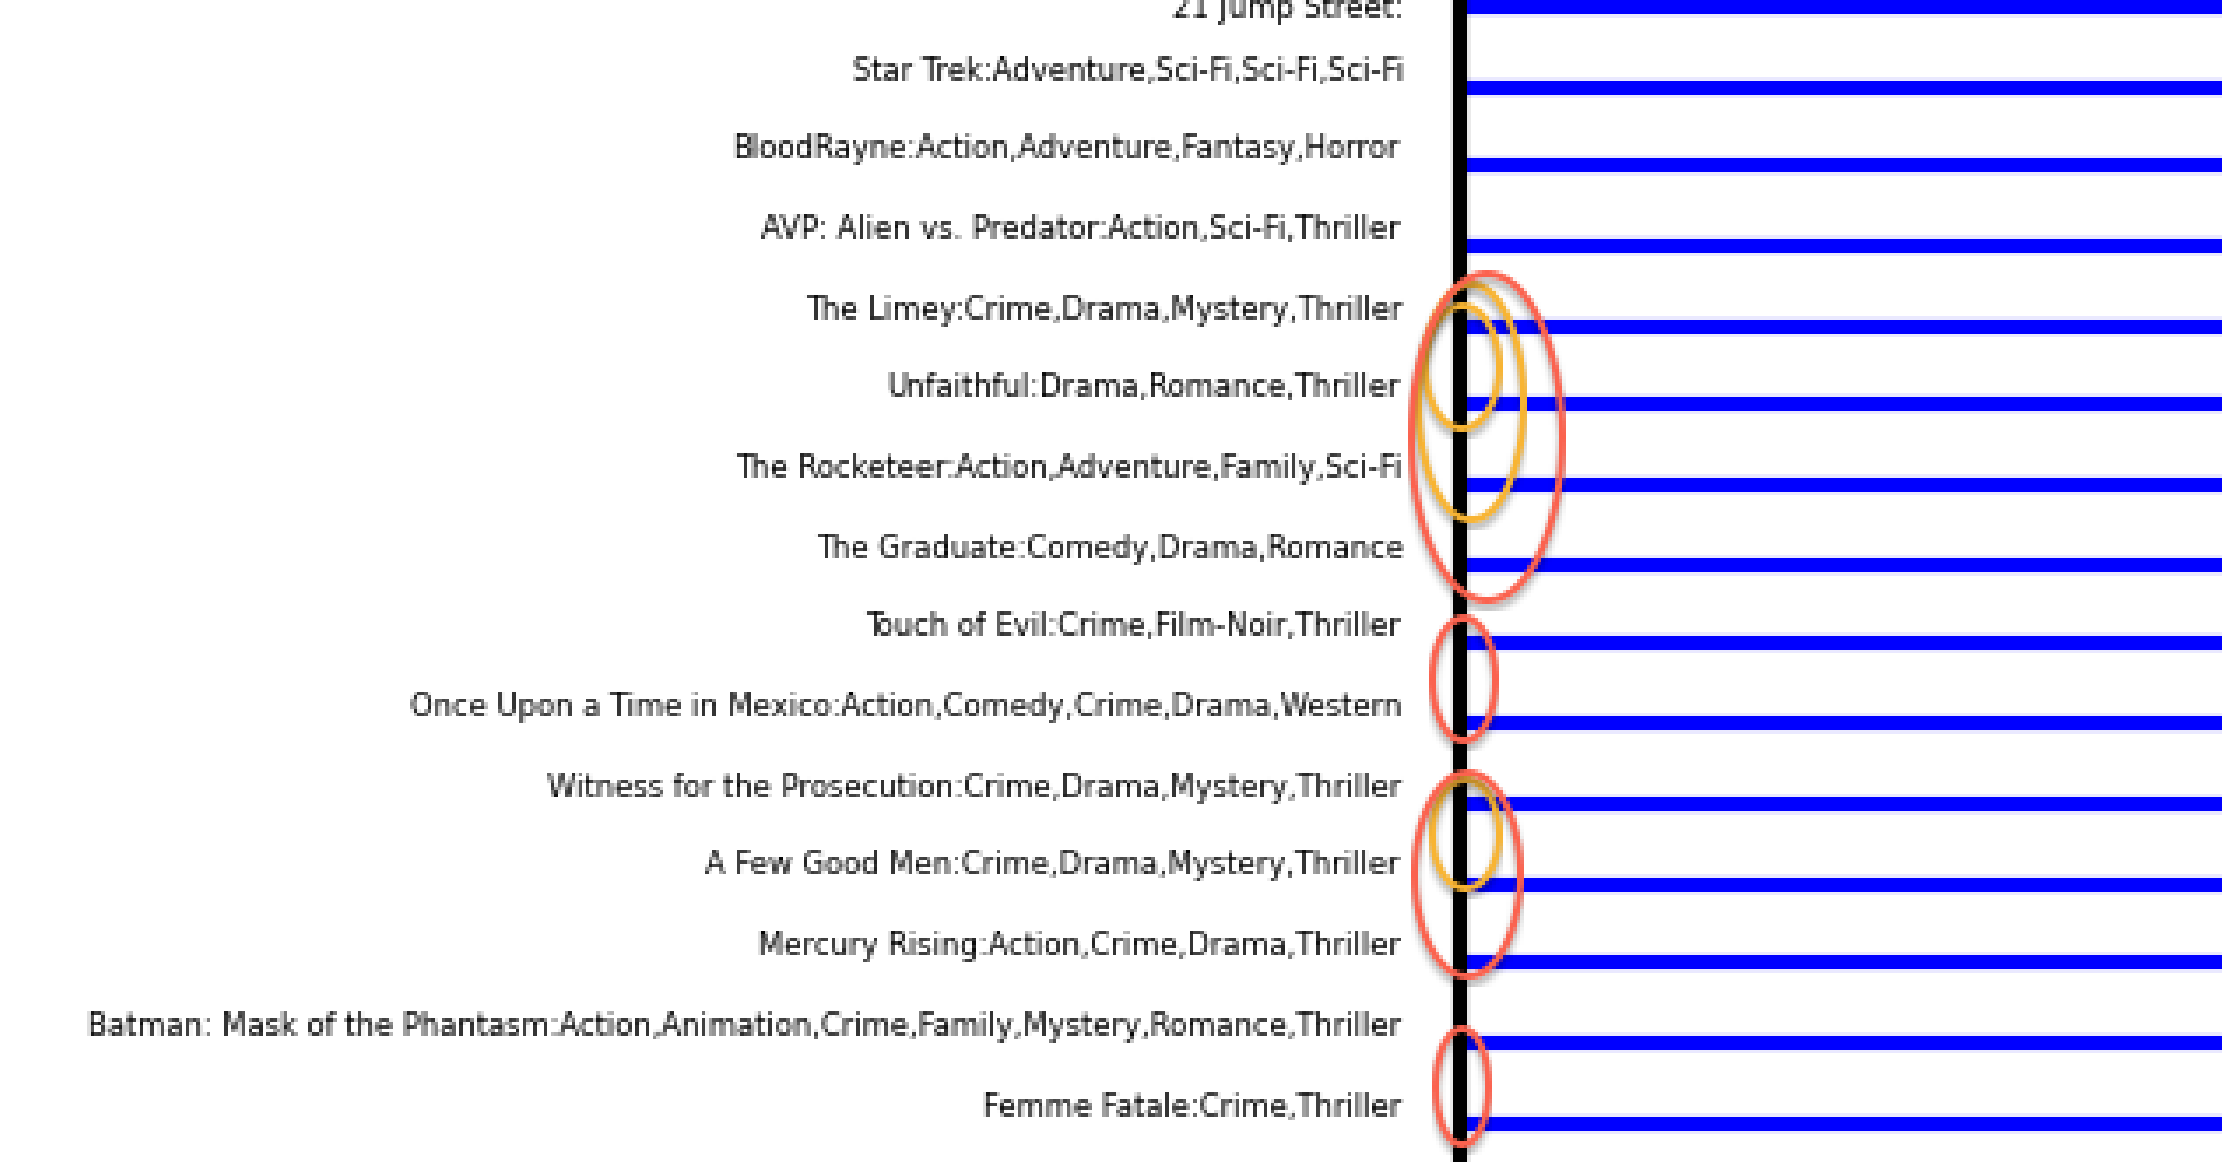
\includegraphics[width=1\linewidth]{img/zoom.png}
		  \caption{Dendogram du hierachical clustering, zoom}
		  \label{zoom}
		\end{figure}
		\newpage
	%Pour les films sans catégorie on peut cette fois les imaginer en regardant le groupement que l'algorithme a fait. Pour le film "Bruno" (figure \ref{bruno}) on peut en ne déduire que c'est similaire à "Chaplin" et qui aura une catégorie similaire a "Biography, Drama" ou peut-être il's ont simplement la description du film similaire. Peut-être aussi de ce deux films sont définissent une nouvelle catégorie. En regardant sur IMDB et en recherchant sur Wikipedia on peut voire qu’effectivement le film Bruno est un comédie drôle qui parle du personnage Bruno. On peut donc confirmer qui appartiens aussi à la catégorie "Biographie".
	%Pour les films sans catégorie on peut cette fois les imaginer en regardant le groupement que l'algorithme a fait. Pour le film "White noise" (figure \ref{whitenoise}) on peut en ne déduire que c'est similaire à "Rounders" et qui aura une catégorie similaire a "Crime, Drama" ou peut-être il's ont simplement la description du film similaire. Peut-être aussi de ce deux films sont définissent une nouvelle catégorie. En regardant sur IMDB et en recherchant sur Wikipedia on peut voire effectivement le film "White noise" est dans les catégories "Drama, Mystery" c'est qui c'est donc vraisemblable avec notre résultats.
	Dans les clusters crée il y a aussi "Scary Movie" qui est groupé avec "Before the Devil Knows Yo're Dead" (figure \ref{scarymovie})qui ont des catégories complètement différents. Mais, si on regarde le synopsis de deux, on peut voire qu’il y a beaucoup de mot qui sont en commun entre les deux films. Plus précisément les deux films ont les mots "Bobby, Ray, kill" avec une fréquence très haute dans le deux synopsis. Ce qui explique leur similarité. Cela est aussi vraisemblable parce que "Scary movie" est en effet un parodie des films d'horreur et ce pour cela que dans le résumé on trouve beaucoup de mot en commun. 	
	 
		\begin{figure}[h]
			  \centering
			    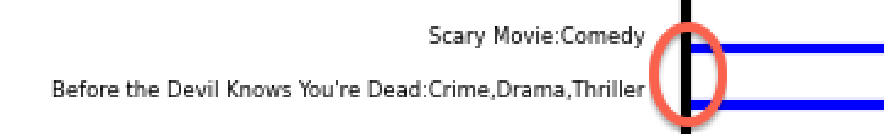
\includegraphics[width=0.5\linewidth]{img/scarymovie.png}
			  \caption{Scary movie et Before the Devil Knows Yo're Dead}
			  \label{scarymovie}
			\end{figure}


	
%---------------------------------------------------------------------------------------------------------------
\section{Map de Kohonen}

Une fois avoir vu que l'algorithme est capable de reconnaitre les films avec une description similaire on peut utiliser un algorithme plus avancé pour avoir en sortie une map des films placés dans une région de la map. Les couleurs de la map représentent la distance entre chaque film. Rouge indique que la distance est grande et bleu indique le contraire.

La figure \ref{map1} montre un exemple d'un map généré avec 100 films.

On peut voir depuis l'image
\begin{figure}[h]
	\centering
	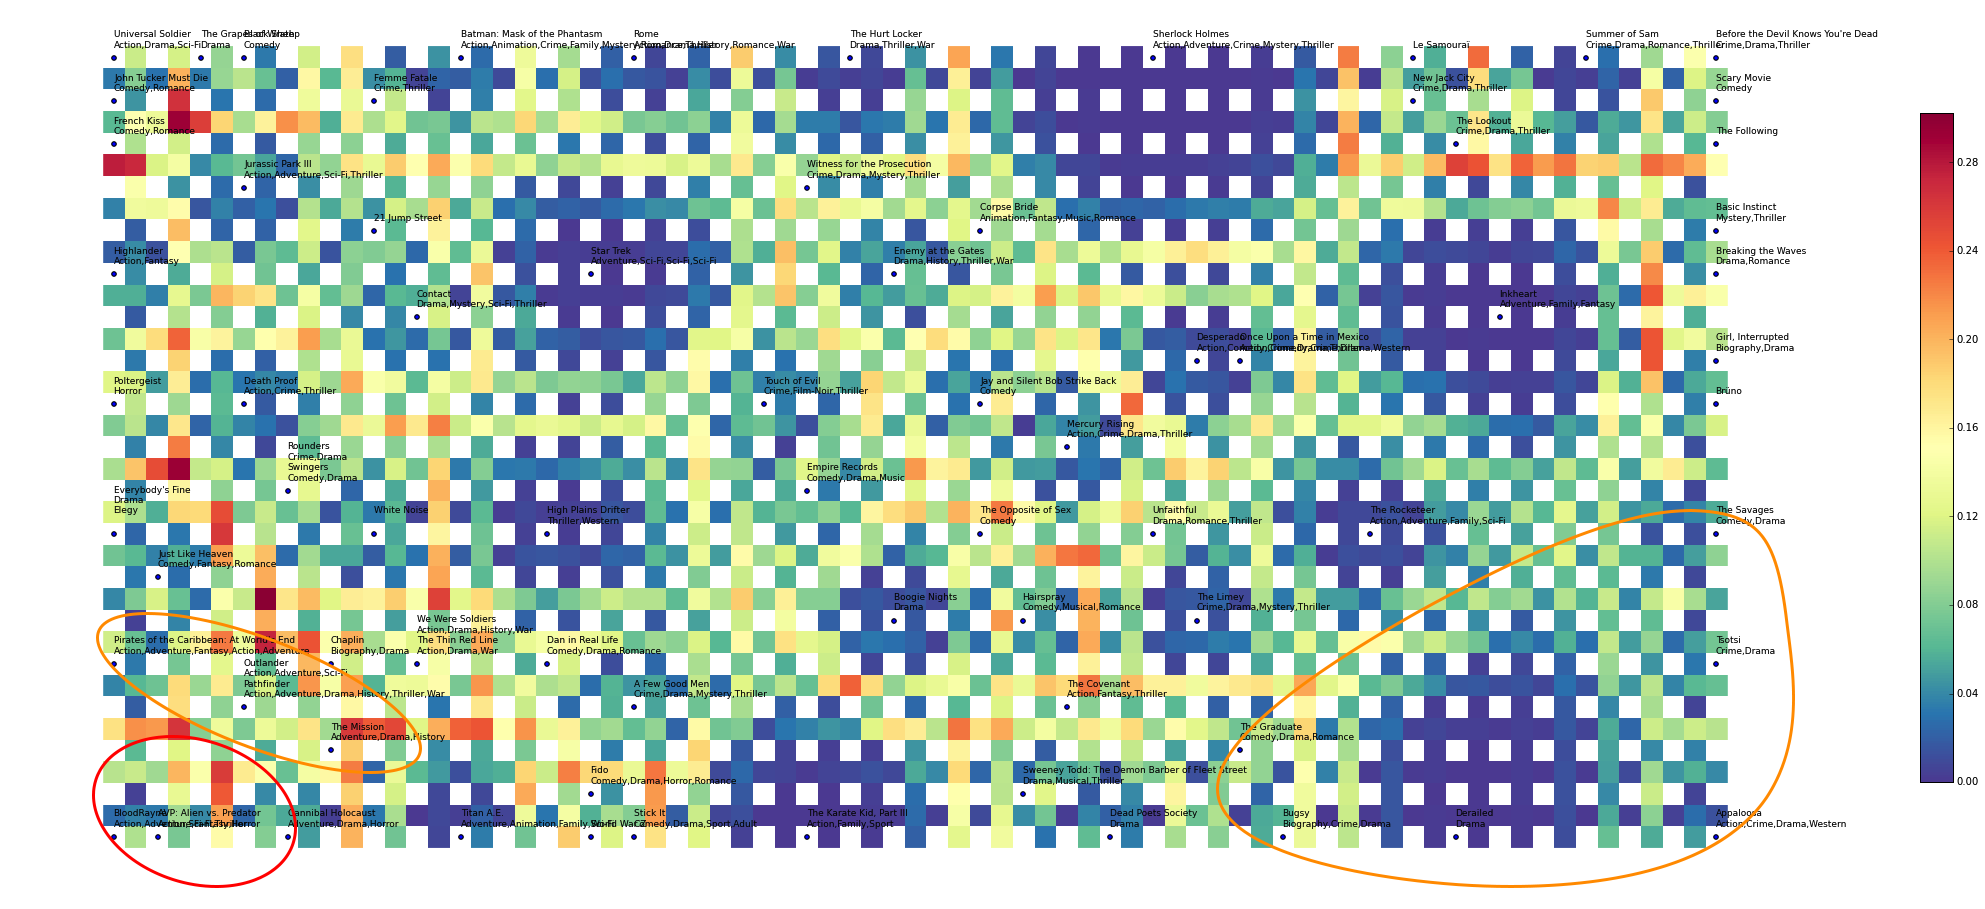
\includegraphics[width=1\linewidth]{img/map-cluster.png}
	\caption{Map de Kohonen avec 100 films}
	\label{map1}
\end{figure}

On peut voire depuis les couleurs de l'image qui il a de zones délimitées par de rouge, comme l'angle en bas à gauche. Il y a aussi des zones délimitées par de vert ou jeune. La division en rouge indique que la division est beaucoup plus forte que celle jeune. Si on agrandit l'image on pourra voir le groupe des films similaire que la map de Kohon a créé.
Dans l'image agrandi (figure \ref{map1zoom2}) on peut voire queil y a des groupes dans l'angle en bas à gauche. On peut voire que l'algorithme mis dans l'angle en bas (cercle rouge) les "Bloody Rayne" et "Alien vs Predator" avec des categorie en comune. On peut en déduire que la description de ce deux est effectivement similaire.

Dans l'ellipse orange on peut voie un outre groupe résultant depuis la map de Kohonen qui met ensemble le filme d'action, d'aventure et dramatique.
\begin{figure}[h]
	\centering
	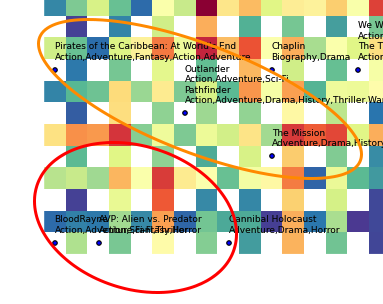
\includegraphics[width=0.5\linewidth]{img/map1zoom2.png}
	\caption{Map de Kohonen avec le zoom de l'angle en bas à gauche}
	\label{map1zoom2}
\end{figure}

Dans l'outre coté de l'image(figure \ref{map1zoom3} ) on peut voire une outre groupe des films. On voit que cette fois on regroupe les films avec les catégories "Crime , Drama, Comedy, Biography". Même si les catégorie sont légèrement différentes on doit pense que la reconnaissance est fait sur la description du film et pas sur d'autre paramètre plus a haut niveau.

\begin{figure}[h]
\centering
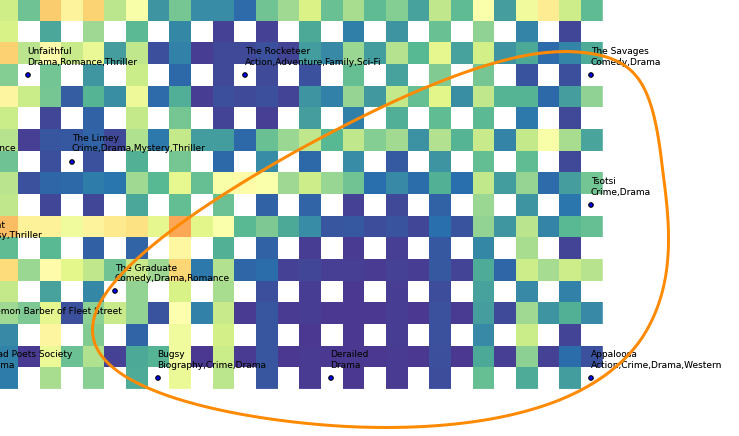
\includegraphics[width=0.6\linewidth]{img/map1zoom3.png}
\caption{Map de Kohonen avec le zoom de l'angle en bas à droite}
\label{map1zoom3}
\end{figure}


%---------------------------------------------------------------------------------------------------------------
% Code integration example
%\begin{lstlisting}[language=bash]
%  sudo apt-get update
%  sudo apt-get install drupal7
%\end{lstlisting}

% Image integration example
%\begin{figure}[h]
%  \centering
%    \includegraphics[width=1\linewidth]{img/drupalFirstPage.png}
%  \caption{Page d'accueil du site créé avec Drupal sur une instance EC2}
%  \label{drupalfirstpage}
%\end{figure}

% Image side-by-side
%\begin{figure}[h!]
%    \centering
%    \begin{tabular}{cccc}
%      \includegraphics[width=.14\linewidth]{randomTree_n5.png} &
%      \includegraphics[width=.22\linewidth]{randomTree_n10.png} &
%      \includegraphics[width=.22\linewidth]{randomTree_n15.png} \\
%      (a) & (b) & (c)\\
%    \end{tabular}
%    \caption{Arbres aléatoires où (a) n=5 (b) n=10 (c) n=15
%    \label{randomTrees}}
%\end{figure}
\chapter{Perspectives et améliorations}
%---------------------------------------------------------------------------------------------------------------
\section{Optimisations supplémentaire de la matrice}

Comme dit dans la partie résultats, il y a des mots qui apparaîssent vraiment souvent dans beaucoup de textes, il faudrait détecter ceux qui sont importants et supprimer les autres. Cela ferait gagner du temps à l'exécution et optimiserait la catégorisation. Il s'agit là de peu de mots, qui apparaîssent vraiment souvent.

Ensuite il y a autre chose qui peut être amélioré. Lors de l'optimisation, nous supprimons tous les mots qui apparaîssent une seule fois dans tous les textes. Il faudrait maintenant également supprimer les mots qui apparaîssent plusieurs fois, mais uniquement dans un texte. En effet, des mots qui sont uniquement dans un seul film ne permettent pas de faire des comparaisons avec les autres films donc ils servent à rien.

%---------------------------------------------------------------------------------------------------------------
\section{Prise en compte de plus d'informations relatives aux films}

Pour améliorer encore la catégorisation, il serait possible d'aller chercher les descriptifs de films sur d'autres sources, telles que Wikipédia par exemple. Avec des textes plus longs pour chaque film, la catégorisation serait certainement meilleure.

En étandant le concept, il pourrait être intéressant d'ajouter à la classification les sous-titres complets des dialogues du film. Dans ce cas, il faudrait certainement appliquer les mêmes traitements sur les mots que ce que nous avons fait jusque là.

Jusque là, la catégorisation est sensée être objective et logique puisqu'elle est basée sur les données du film lui-même. Mais nous pourrions imaginer ajouter à ça une classification émotionnelle des personnes qui ont vu le film en ajoutant à la reconnaissances différentes informations : \\

\begin{itemize}
 \item les critiques sur le film sur IMDb
 \item les commentaires sur le film sur Facebook
 \item les tweets relatifs au film sur Twitter
 \item les reviews sur le film tirées de différents blogs
\end{itemize}

\vspace{0.4cm}

Une autre classification qui pourrait être intéressante et de classifier les films en fonction des acteurs. Cela nous montrerai les différents films où plusieurs acteurs jouent en même temps par exemple. Ajouter la date de production du film peut également être intéressant.

%---------------------------------------------------------------------------------------------------------------
\section{Dynamiser la classification}

Actuellement, nous pouvons entrer le nom d'un film dans une méthode en Python, et les dix films les plus ressemblants sont affichés. Ce système implique que le film soit déjà contenu dans la classification. On pourrait imaginer un système qui, lorsque le nom d'un film est entré, va chercher toutes les informations liées à ce film dynamiquement et refasse la classification pour donner le résultat à l'utilisateur. Cela donnerait un peu de valeur à ce logiciel.

De plus, il faudrait mettre en place un site web permettant de faire les recherches de manière intuitive et avec un beau design pour le mettre en avant.


%---------------------------------------------------------------------------------------------------------------
% Code integration example
%\begin{lstlisting}[language=bash]
%  sudo apt-get update
%  sudo apt-get install drupal7
%\end{lstlisting}

% Image integration example
%\begin{figure}[h]
%  \centering
%    \includegraphics[width=1\linewidth]{img/drupalFirstPage.png}
%  \caption{Page d'accueil du site créé avec Drupal sur une instance EC2}
%  \label{drupalfirstpage}
%\end{figure}

% Image side-by-side
%\begin{figure}[h!]
%    \centering
%    \begin{tabular}{cccc}
%      \includegraphics[width=.14\linewidth]{randomTree_n5.png} &
%      \includegraphics[width=.22\linewidth]{randomTree_n10.png} &
%      \includegraphics[width=.22\linewidth]{randomTree_n15.png} \\
%      (a) & (b) & (c)\\
%    \end{tabular}
%    \caption{Arbres aléatoires où (a) n=5 (b) n=10 (c) n=15
%    \label{randomTrees}}
%\end{figure}
\chapter{Conclusion}
%\section{Conclusion}




\vspace{1cm}
Fribourg, le \today

\vspace{0.2cm}

\hspace{2cm} Simone \textsc{Cogno} \hspace{5cm} Jacky \textsc{Casas}

\vspace{2cm}

%\newpage

%\appendix % annexes
%\chapter{Code source}
% \section{}


\end{document}
